\chapter{Inledning}

En drönare är ett obemannat luftfordon som kan styras med hjälp av visionsbaserad-, tröghets- eller satellitnavigation \citep{geospatial}. För att robotar eller drönare skulle kunna navigera autonomiskt måste den vara medveten om sitt läge, omgivning, hastighet, kursriktning samt start- och slutplats. Andra faktorer som borde beaktas för att flyga från start till slutplatsen är hur drönare kan behandla data från inbyggda sensorer i sig, det vill säga kartlägga miljön och sin egen position i denna miljö samt hur man planerar vägen utan att kollidera med hinder.

För att drönare är mer versatila än robotar som inte flyger så finns det mera användningsfall för dem. De kan övervaka markföroreningar, industriolyckor eller växternas behov av vatten och näring \citep{crowdsurveillance}. Drönare har också använts vid katastrofområden, såsom vid Japans jordbävning för att mäta strålningsvärden i Fukushima och få visuell information om katastrofområdet samt räddning av invandrare vid medelhavet. I logistik är man också intresserad om autonoma drönaren som skulle leverera paket för kunder, till exempel 86 \% av Amazons paket väger mindre än 5 skålpund (ca. 2.26 kg) \citep{cbsnews}. Mest lovande forskning är inom vision baserad navigering med hjälp av datorseende.

Robotnavigering med hjälp av datorseende är ett aktivt forskningsområde \citep{982903}. För att robotar skulle vara verkligen autonomiska måste de kunna kartlägga sin omgivning och lokalisera sig själv i omgivningen, detta kallas för SLAM (Simultaneous Localization and Mapping). SLAM är ett problem som har fått uppmärksamhet av det vetenskapliga samfundet sedan 80-talet och har sätts som ett rön om det löses. Utmaningar i utvecklingen är att konstruera algoritmer som fungerar i allmänhet, såsom i dynamiska och stora miljön \citep{realslamproblem}.

Avhandlingen kommer att vara en översikt om SLAM problemet och vilka metoder det finns för att kartlägga miljön och lokalisera sig själv med hjälp av datorseende. Frågor som behandlas är: Vad är det fundamentala problemet med SLAM? Vilka SLAM metoder skulle kunna användas eller har använts med drönare och vad begränsar användningen av dessa? Varför har vision baserad navigation fått så mycket uppmärksamhet än de traditionella metoderna?

Resten av avhandlingen är strukturerad enligt följande: I kapitel 2 öppnas bakgrund bakom navigering, kartläggning, lokalisering och bildbearbetning som är nödvändiga för SLAM, kapitel 3 innehåller information om samtidig lokalisering och kartläggning och hur SLAM problemet kan grupperas i olika kategorier enligt data som man har.

\chapter{Bakgrund}

\section{Navigering}

Med navigering anser vi att en drönare planerar och utför en rutt från startplats till målet \citep{geospatial}. För att kunna navigera till målet måste den vara medveten om sitt läge, miljö, kursriktning och hastighet. Autonomisk navigering kräver att drönare kan undvika hinder, planera sin rutt samt ta omvägar vid behov. I visionsbaserad navigering används visuella sensorer för att få bilder som indata. Bilderna kan sedan behandlas med algoritmer för att få en representation av omgivningen och lokalisera drönare i omgivningen. 

Visuella sensorer som kan användas är monokulära, stereo, RGB-D och fisheye-kameror samt kombinationer av dessa \citep{geospatial}. Kamerasensorer är billiga att operera, väger lite och med dem kan man uppfatta färg, textur och former. Traditionella navigeringsmetoder såsom satellit, som använder GPS-signaler (Global Positioning System) för lokalisering, och tröghetsnavigering (Inerital Navigation System), som använder accelerometer och gyroskop, får man inte visuell information av omgivningen. Med kameror kan man navigera i GPS-förnekade områden för att kameror är passiva, det vill säga de kan inte bli störda av utomstående signaler eller upptäckas av utomstående entitet. 

Drönare kan använda laser och ultraljudsensorer för att navigera men dessa kräver mycket energi och väger mer än kameror \citep{6385934}. För att drönare byggs mindre än förr, och på grund av detta har begränsad bärförmåga samt batterikapacitet, har dessa sensorer uteslutnas. Med hjälp av vision baserad navigering, som använder kameror, kan man få rikligt med information om omgivningen \citep{geospatial}. Visionsbaserad navigering, som är ett aktivt forskningsområde, är den mest lovande metoden inom robotnavigering.

\section{Datorseende och bildbearbetning}

Bildbearbetning i visionsbaserad navigering betyder att man gör utdrag ur bilder i form av former, kanter, linjer, djuphet, rörelse, färg eller mönster \citep{982903}. Man kan också utjämna bilder \citep{mapbuildingsift}. Detta menar att man blurrar bilder för att få bort brus och då man gör utdrag ur bilder i form av egenskaper får man färre, men bättre träffar. Metoder för att uppskatta djuphet med datorseende är att beräkna binokulära skillnaden eller rörelseparallax \citep{suomimainittu}. 

Rörelseparallax betyder att objekt rör på sig snabbare då de är närmare observatören och långsammare då de är långt borta. För att räkna binokulära skillnaden behöver man två kameror som är riktade parallellt i samma linje, kamerornas distans från varandra är känd, deras synfält överlappar och av båda kamerornas bilder utdras samma kännetecken \citep{suomimainittu}. Från skillnaden ur landmärkets horisontala position i båda av kamerornas bilder kan man estimera djuphet. Med en monokulär kamera kan man uppskatta djuphet av bilder baserat på rörelseparallax. För att bygga djuphetskarta med monokulärkamera och rörelseparallax behöver man veta distansen till ett objekt då navigeringen börjar och som indata får man bilder och rörelseinformation av roboten \citep{suomimainittu}. \cite{suomimainittu} undersökte detta och märkte att stereokameror fungerar bättre då objekten är nära medan monokulära kameror med hjälp av rörelseparallax kan uppfatta mer precis distans då distansen växer. 

För att få former, kanter eller linjer ur bilder finns det olika algoritmer såsom SIFT (Scale-Invariant Feature Transform), HARRIS hörn upptäckare, SURF (Speeded Up Robust Features), ORB (Oriented FAST and Rotated BRIEF), med mera \citep{orb, slamproblem, mapbuildingsift}. SIFT, SURF och ORB prövar hitta egenskaper från bilderna som är invariant för rotation, som menar att samma egenskaper kan hittas från olik synvinkel \citep{orb}. Enligt \cite{orb} är ORB mer energieffektiv än SIFT för att den kräver mindre beräkning för att hitta egenskaper, som menar att den är snabbare färdig utan att tappa effektivitet.

\section{Lokalisering i omgivningen}

Med att en robot lokaliserar sig själv menar vi att den tar reda på sin position i miljön \citep{982903}. Då man har en uppfattning om miljön, det vill säga en karta, så kan en drönare lokalisera sig själv med att ge den landmärken som den hittar då den navigerar eller så kan den observera dessa själv och associera dem med kartan som den har. Från bilderna ur kamerorna i drönaren identifieras landmärken, sedan matchas observerade landmärken med de som finns i kartan och efter det kan man estimera positionen av roboten.

Positionen och orientationen av roboten beräknas med sannolikhetsberäkning baserat på tid och indata av sensorer \citep{ProbabilisticRobotics}. Då vi lokaliserar en robot så är roboten vid någon plats, den rör på sig och sedan observerar landmärken. Om man betecknar tiden för varje tidpunkt med $t$, så då betecknas robotens position och riktning med $x_t$, rörelseinformation av roboten med $u_t$ och landmärken extraherade från kamerasensorer med $z_t$. För att $x_t$ är en möjlighet i en kontinuerlig stokastisk variabel $X$ så kan betingade sannolikhetsfördelningen för $x_t$ skrivas som följande:

\begin{align}
    P( X = x_t | x_{0:t-1}, z_{1:t-1}, u_{1:t})
\end{align}

Där vi antar att roboten rör på sig $u_1$ före den skaffar sensorinformation $z_1$. Med Markovegenskapen för $x_t$, som betyder att en villkorlig sannolikhetsfördelning för $x_t$ är bara beroende på den tidigare sannolikhet $x_{t-1}$ och inte på händelseförloppet som hände före $x_{t-1}$. Då $x_t$ är den bästa framtidssyn så kan vi begränsa att $x_t$ är beroende bara på den tidigare position $x_{t-1}$ och rörelseinformation $u_t$, se figur \ref{markov}. Betingade sannolikhetsfördelningen för $x_t$ kan då betecknas som följande:

\begin{align}
    P(x_t | x_{t-1} u_{t})
\end{align}

Om $x_t$ har Markovegenskapen så då är betingade sannolikhetsfördelningen för observerade landmärken $z_t$:

\begin{align}
    P(z_t | x_{0:t}, z_{1:t-1}, u_{1:t}) = P(z_t|x_t)
\end{align}

\begin{figure}[ht]
    %\begin{figure}[tbh] t= top, b = bottom, h=here
    \begin{center}
    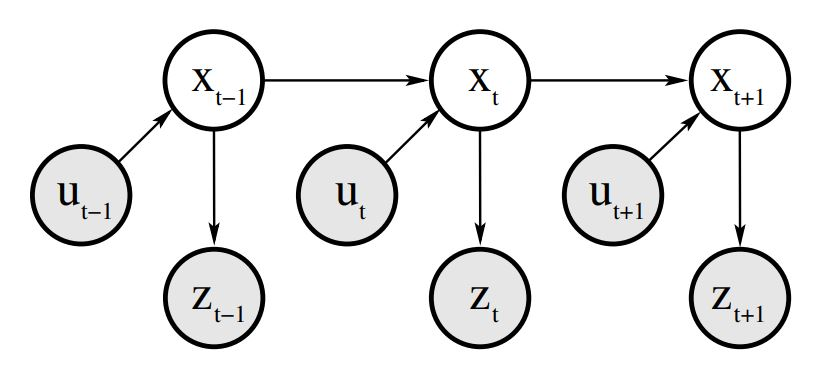
\includegraphics[width=0.75\textwidth]{markov.JPG}
    \caption{En graf om lokalisering som visualiserar Markovegenskapen där till exempel $x_t$ är bara beroende av $x_{t-1}$ och $u_t$ \citep{ProbabilisticRobotics}.}
    \label{markov}
    \end{center}
\end{figure}

$P(x_t|x_{t-1}, u_{t})$ är rörelseuppfattningssannolikhet och $P(z_t|x_t)$ är landmärkesuppfattningssannolikhet för roboten \citep{ProbabilisticRobotics}. 

Positionen och riktning av roboten kan beräknas med Bayes filter \citep{ProbabilisticRobotics}. Bayes filter är en rekursiv algoritm som beräknar aposteriorisannolikhet för robotens position $bel(x_t)$ baserat på robotens tidigare position $bel(x_{t-1})$, rörelseinformation $u_t$ och observerade landmärken $z_t$. Med hjälp av Bayes regler, lagen om total sannolikhet för kontinuerliga variabler och Markovegenskapen kan detta bevisas med matematisk induktion där vi antar att $x_t$ har Markovegenskapen och att $bel(x_0)$ täthetsfunktion är känd då $t = 0$. Med att täthetsfunktionen är känd menar vi att roboten vet sin position vid början med full säkerhet eller så är $bel(x_0)$ en likformig sannolikhetsfördelning.
\begin{align}
bel(x_t) & = P(x_t | z_{1:t}, u_{1:t}) \tag{BF1}\label{BF1} \\
        & = \eta P(z_t | x_t, z_{1:t-1}, u_{1:t}) P(x_t | z_{1:t-1}, u_{1:t}) \tag{BF2}\label{BF2}\\
        & = \eta \underline{P(z_t | x_t)} P(x_t | z_{1:t-1}, u_{1:t}) \tag{BF3}\label{BF3}\\
        & = \eta P(z_t | x_t) \underline{\int P(x_t | x_{t-1}, z_{1:t-1}, u_{1:t}) P(x_{t-1} | z_{1:t-1}, u_{1:t}) dx_{t-1}} \tag{BF4}\label{BF4}\\
        & = \eta P(z_t | x_t) \int \underline{P(x_t | x_{t-1}, u_t)} P(x_{t-1} | z_{1:t-1}, u_{1:t}) dx_{t-1} \tag{BF5}\label{BF5}\\
        & = \eta P(z_t | x_t) \int P(x_t | x_{t-1}, u_t) P(x_{t-1} | z_{1:t-1}, \underline{u_{1:t-1}}) dx_{t-1} \tag{BF6}\label{BF6}\\
        & = \eta P(z_t | x_t) \int P(x_t | x_{t-1}, u_t) \underline{bel(x_{t-1})} dx_{t-1} \tag{BF7}\label{BF7}
\end{align}
Bayes filters definition är \ref{BF1}, det vill säga förtroende för roboten att den är vid $x_t$, som betecknas $bel(x_t)$, är samma som sannolikheten av $x_t$ givet $z_{1:t}$ och $u_{1:t}$. Med Bayes teorem kan detta skrivas om i format \ref{BF2}. Vid \ref{BF3} använder vi Markovegenskapen för $x_t$ så kan betingade sannolikheten för $z_t$ skrivas som landmärkesuppfattningssannolikheten. Med satsen om total sannolikhet för kontinuerliga variabler, som uttrycker sannolikhet för enskilda händelser till betingade sannolikhet, kan formeln skrivas om till \ref{BF4}. Vid \ref{BF5} och \ref{BF6} använder vi Markovegenskapen för $x_t$, se figur \ref{markov}. Till slut får vi \ref{BF7}, som bevisar med induktion att algoritmen fungerar rekursivt \citep{ProbabilisticRobotics}.

Bayes filters algoritmen fungerar så att för varje $x_t$ beräknas två kritiska steg, som är spådom och korrigering \citep{ProbabilisticRobotics}. Spådomsdelen i algoritmen är delen där vi beräknar integralen för två faktorer: sannolikheten att rörelseinformationen $u_t$ tar oss till $x_t$ och den gamla förtroende av positionen $bel(x_{t-1})$. Korrigeringsdelen är då man multiplicerar spådomsdelen med sannolikhet att $z_t$ skulle observeras för varje möjliga $x_t$. Oftast är korrigeringsdelen inte en sannolikhet, alltså täthetsfunktionens summa är inte 1 för varje värde, så därför används det en normering konstant $\eta$ för att normera sannolikheten. Ett steg av algoritmen är definierat nedan som sedan görs rekursivt för resultatet av algoritmen och när man har ny rörelseinformation och landmärken.

\begin{algorithm}[H]
    \SetAlgoLined
    \SetAlgoRefName{BFA}
    \label{BFA}
    \FuncSty{BayesFilter($bel(x_{t-1})$, $u_t$, $z_t$):} \\
    \ForAll{$x_t$}{
        $spådom$ = $\int P(x_t | x_{t-1}, u_t) bel(x_{t-1}) dx_{t-1}$ \\
        $bel(x_t)$ = $\eta P(z_t | x_t)$ $spådom$
    }
    \Return{$bel(x_t)$}
    \caption{Bayes Filter Algoritm}
\end{algorithm}

Bayes filter är huvudsakliga algoritmen för att beräkna robotens position och riktning \citep{ProbabilisticRobotics}. Algoritmen baserar sig starkt på Markovegenskapen att det nuvarande läge är oberoende av tidigare data. I robotnavigering är det inte dock så lätt att anta detta, för det skulle betyda att allt runtomkring roboten borde vara statiskt. Till exempel om en bil rör på sig då roboten navigerar så då man gör landmärkesuppfattning kommer Bayes filter att ge felaktig estimering. Bayes filtern är också basis för många andra lokaliseringsalgoritmer, som till exempel Kalman filter eller Markov lokalisation. 

Positionen av roboten kan beräknas också utan kartan med att räkna distansen till landmärken och distansen mellan landmärken som extraheras ur bilder \citep{realslamproblem}. Lokalisering kan delas i global och lokal lokalisering \citep{982903, globalsubmaps}. Med global lokalisering har roboten ingen vetskap om sin position i början av navigeringen. I lokal lokalisering har roboten en ungefärlig eller exakt vetskap om sin plats vid början av navigeringen som den fått som indata. Lokala lokaliseringsmetoder strävar för att korrigera fel som uppstår av robotens rörelse. Globala lokaliseringsmetoder kan återvinna från verkliga misstag då man estimerar robotens position.

\section{Kartläggning av omgivningen}

En karta om miljön kan representeras i två (2D) eller tre (3D) dimensioner \citep{geospatial}. Kartor kan sparas i olika format, såsom datorstödd konstruktion (CAD, Computer-Aided Design), beläggningskarta (Occupancy Map), topologisk karta eller en enkel graf om landmärken och deras sammankopplingar \citep{982903}. En datorstödd konstruktion av miljön kan vara en mycket detaljerad representation av omgivningen. En beläggningskarta är en 2D eller 3D-modell av omgivningen som är sparat i ett rutsystem där rutor som är upptagna är någon objekt i miljön \citep{6095058, 982903}. 

Kartan kan vara färdigt sparad för en drönare eller så kan miljön kartläggas från bilderna av sensorerna då den flyger \citep{geospatial}. Med 3D volymetriska sensorer kan man konstruera en 3D modell och spara denna information i en Octree-struktur. Med strukturen kan data om miljön packas i mindre format utan att tappa möjligheten att uppdatera informationen vid behov. En annan metod som tas upp är med stereovisionsalgoritmer göra en djuphetskarta och behandla data till plana ytor som minskar på missvisning som uppstår med användning av stereovision algoritmer när man bygger upp djuphetskartan.

\chapter{Samtidig lokalisering och kartläggning}

Samtidig lokalisering och kartläggning (SLAM) är ett av de grundläggande problem i robotnavigering \citep{realslamproblem}. SLAM är ett problem där en autonom robot som inte har tidigare information om sin plats eller omgivning skall samtidigt bygga en karta och lokaliserar sig själv till exempel med hjälp av att identifiera landmärken. Detta kan estimeras med sannolikhetsberäkning baserat på tid $k$, där man tar i beaktande riktningen och positionen av roboten $x_k$, distansen roboten rör på sig $u_k$, landmärken som är invariant för rörelse $m_i$ och observationer för varje landmärke $i$ som roboten gör vid varje tidpunkt $z_{ik}$, se figur \ref{slam-problemet}. Några lösningar för SLAM som baserar sig på sannolikhetsräkning är Extended Kalman Filter (EKF-SLAM) och FastSLAM \citep{realslamproblem}. 

\begin{figure}[ht]
    %\begin{figure}[tbh] t= top, b = bottom, h=here
    \begin{center}
    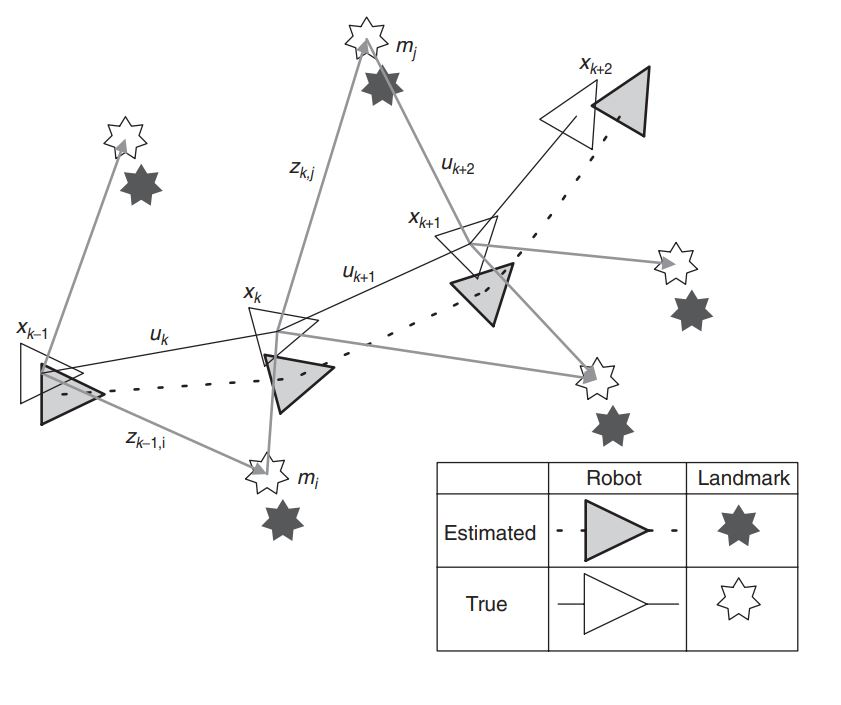
\includegraphics[width=0.75\textwidth]{slam-problem.JPG}
    \caption{Bild på SLAM-problemet \citep{realslamproblem}.}
    \label{slam-problemet}
    \end{center}
\end{figure}

SLAM-problemet har delproblem som borde lösas för att få robotar att navigera autonomiskt \citep{slamproblem}. Det svåraste problemet i flesta SLAM-lösningar är dataföreningsproblemet som betyder att man identifierar två olika landmärken som en och samma. Detta problem kan uppstå redan vid korta rörelsen av robotar eller då en robot har navigerat och kommer till en plats som den har redan varit i förr, detta kallas för loopstängning (Loop Closure). Med att förena landmärken fel så uppkommer det missvisningar då man estimerar positionen av roboten.

För autonom navigering behöver en robot veta sitt läge i miljön \citep{geospatial}. Med hjälp av kameror, bildbearbetning och beräkning kan miljön kartläggas, i helhet eller delvis, och drönaren lokalisera sig själv, detta kallas också för visuell lokalisering och kartläggning. Detta kan delas i tre kategorier, som är kartlösa (mapless), kartbaserade (map-based) och kartbyggande (map-building) system. 

\section{Kartlösa system}

I system utan karta navigerar drönare bara med hjälp av att observera tydliga egenskaper i miljön \citep{982903}. Dessa kan vara till exempel väggar, dörrar, möbler eller andra landmärken. Metoder som används inom kartlösa system är optiskt flöde (Optical flow) och spårning av egenskaper (Feature tracking). 

\subsection{Optiskt flöde}

Santos-Victor et. al har använt optiskt flöde i en robot för att imitera bin \citep{341094}. De placerade två kameror på varsin sida av en robot och beräknade hastigheten från bilderna av båda kamerorna med att ta fem bilder som utjämnas med Gaussisk oskärpa och de två sista utjämnade bilder används för att beräkna medeltalet av optiska flödesvektorer. Om flödesvektorerna var samma på båda sidorna så for roboten rakt framåt, annars så far den mot den sida vilkens hastighet är mindre. Metoden som Santos-Victor et al. använde för roboten fungerar bara om båda kamerorna är symmetriskt riktade från varandra när man tar i beaktande rörelseriktningen av roboten \citep{982903}. Denna teknik fungerar dåligt i texturlösa miljö och det går inte att byta rörelseriktningen. Fastän metoden som \cite{341094} använde tog bara i beaktande horisontala flödesvektorer så har sedan detta användning av optiska flödesmetoder forskats mera. Nuförtiden kan man använda drönare för att uppskatta avstånd, hålla sin höjd, undvika hinder, beräkna hastighet och landa på en plattform som rör på sig med hjälp av optiskt flöde \citep{6564752}.

\subsection{Spårning av egenskaper}

Spårning av egenskaper (Feature tracking) används för att skaffa information om objekt, så som linjer, hörn och olika former som är invariant för rörelse \citep{geospatial}. Med hjälp av dessa egenskaper av objekten och deras relativa rörelse i sekventiella bilder kan man bestämma robotens position. Då drönare navigerar i området, så kommer den troligtvis att se dessa objekt från olika perspektiv, som hjälper drönare att navigera. Traditionella SLAM-lösningar, såsom EKF-SLAM och FastSLAM faller under denna kategori \citep{voslamlatif}. Dessa SLAM-lösningar fungerar inte då det finns mycket egenskaper att extrahera i miljön. EKF-SLAM nackdel är beräkningsbehovet som växer kvadratiskt och FastSLAM nackdel är bildprocessering. 

För att drönaren har begränsad batterikapacitet och bärkraft har \cite{voslam} föreslagit användning av VO-SLAM (Visual Odometry SLAM) som kan kartlägga omgivningen och lokalisera observatören då det finns upp till 30 000 egenskaper i kartan, med en stereokamera som tar 31 bilder per sekund och en krets som använder tio gånger mindre energi än en Intel i7 3770K-processor \citep{voslam}. Deras VO-SLAM algoritm implementeras i en FPGA-krets (Field-Programmable Gate Array) vilkens logik är omprogrammerbar, den använder färre energi än vanliga processorer och kan beräkna parallellt. 

VO-SLAM-lösningen fungerar så att de extrahera landmärken med SIFT från bilderna \citep{voslam}. Med hjälp av binokulära skillnaden från bilderna i stereokameran konstruera de en 3D-representation av dessa landmärken som de sparar i en matris. FPGA-kretsen, som är programmerat för matrisberäkning, beräknar vektorvinklarna för varje observerade landmärke från globala kartan och hittar de bästa träffar för lokaliseringsalgoritmen. Före lokaliseringsuppfattningen använder de RANSAC (Random Sample Consensus) för att ta bort avvikande träffar inom landmärken, se figur \ref{voslamprocess}. 

\begin{figure}[ht]
    %\begin{figure}[tbh] t= top, b = bottom, h=here
    \begin{center}
    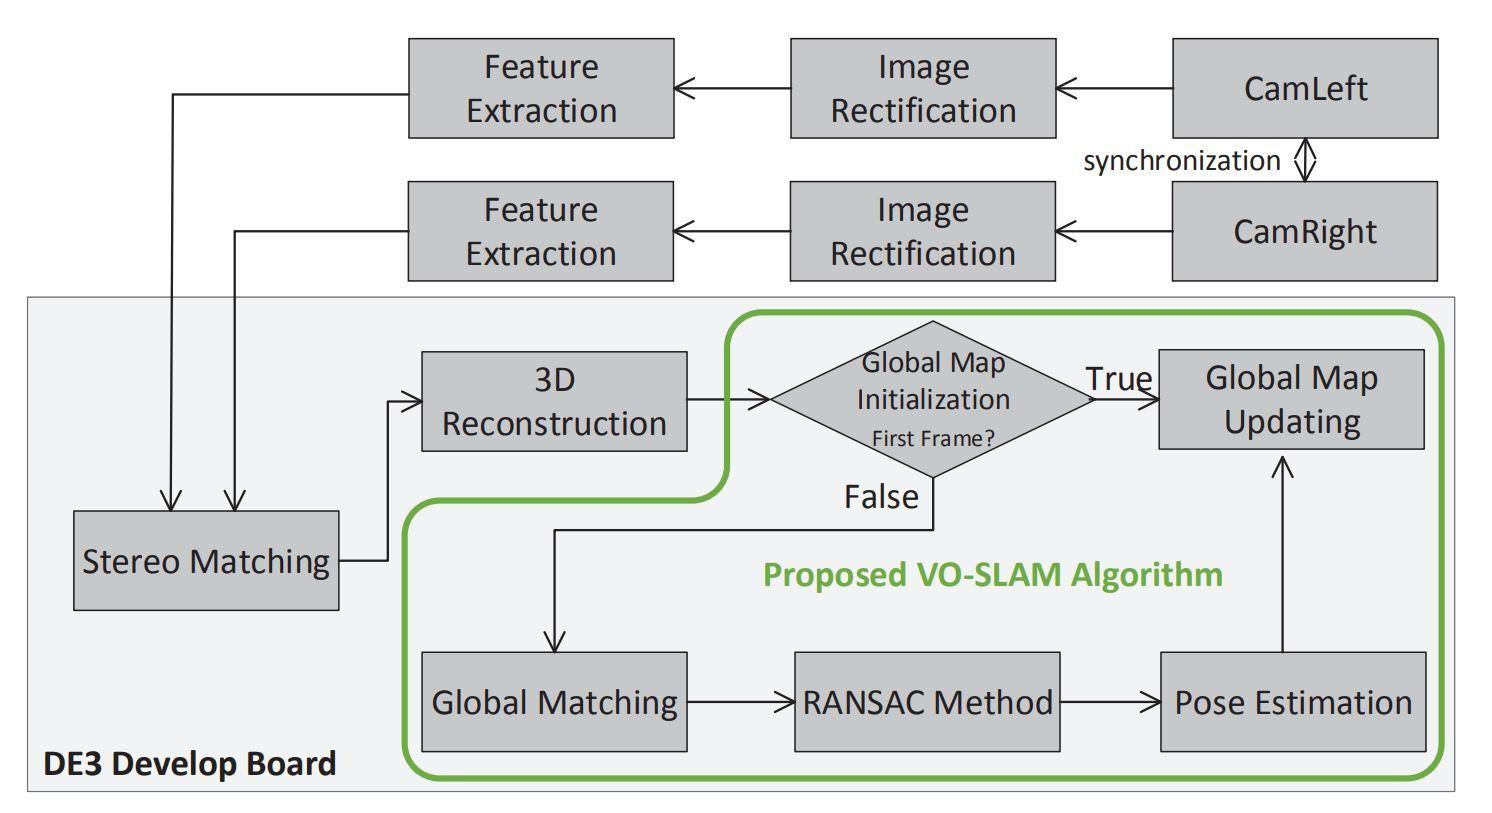
\includegraphics[width=0.75\textwidth]{voslam.JPG}
    \caption{Bild på VO-SLAM processen \citep{voslam}.}
    \label{voslamprocess}
    \end{center}
\end{figure}

Med hjälp av FPGA-kretsen har de fått dataförening med matriser att beräknas i realtid med upp till 31 bilder i sekund och litet energibehov. Enligt \cite{voslam} kan VO-SLAM estimera positionen med 1–2 cm exakthet med upp till 30 000 landmärken i kartan, hantera loopstängning och är mest energieffektiva lösningen \citep{voslam}. Något som deras lösning tar inte i beaktande är SIFT algoritmens tidkrav. \cite{voslamlatif} använder VO-SLAM där de delat upp processen så att indata från stereokameran, bildbearbetning och 3D-representationen som görs med SIFT bearbetas i en egen processor och uppdatering av kartan, matcha observerade landmärken med kartan, lokalisering och uppdatering av kartan hanteras i FPGA-kretsen \citep{voslamlatif}. 

\section{Kartbaserade system}

Med kartbaserade system har drönare en färdig vetskap om miljön som kan vara i form av geometriska modeller, topologiska kartor eller förhållande mellan landmärken \citep{982903}. Idén är att då roboten navigerar prövar den hitta landmärken från bilder som är lika till de landmärken som roboten vet om. När den hittat dessa så kan roboten beräkna sin position i miljön. Med hjälp av karta kan drönare planera sin rörelse i förhand och ta omvägar där det behövs \citep{geospatial}. 

Kartbaserad lokalisering med datorseende kan delas upp i fyra steg, som är följande \citep{982903}:

\begin{itemize}
    \item skaffa sensorinformation av kamerorna
    \item upptäcka landmärken från informationen med bildbearbetning
    \item matcha observationerna med förväntan
    \item beräkna positionen av roboten
\end{itemize}

Det svåraste steget av dessa är att matcha observationerna med förväntan. Detta kallas för dataföreningsproblemet. Man kan inte med full säkerhet veta robotens position och då är det svårt att matcha landmärken från rätt synvinkel.

Då kartan finns kan man fokusera på lokalisering av roboten \citep{982903}. I global lokalisering måste man lita på att man kan förena observationerna med informationen man har och ta i beaktande osäkerheten med att observationerna kan matcha flera av de landmärken man vet om. Detta problem kan lösas till exempel med Monte Carlo lokalisation eller Markov lokalisation. Monte Carlo lokalisation fungerar så att en robot antar med lika sannolikhet sin position i kartan vid början av navigeringen \citep{montecarlo}. Då roboten rör på sig så observerar den nya landmärken och kan beräkna sannolikheten att hur de landmärken den observerat matchar de landmärken i kartan som den vet om. Markov lokalisationsalgoritmen är nästan identisk till Bayes filtern som presenterades vid \nameref{BFA} \citep{ProbabilisticRobotics}. Som indata används också kartan som man har för att estimera positionen av roboten.

I lokal lokalisering måste lokaliseringsalgoritmen hålla koll på osäkerheten av robotens position då den rör på sig och vänder \citep{montecarlo}. Då osäkerhet av sin position är för stor stannar roboten och beräknar sin position med hjälp av visuell information av bilderna, alltså minskar på osäkerheten.

\section{Kartbyggande system}

Kartbyggande system kan användas då det är svårt att navigera med en existerande karta om omgivningen eller om kartan inte finns, som i katastrofområden \citep{geospatial}. Roboten kan vara medveten eller omedveten om sin position vid början av kartbyggandet \citep{globalsubmaps}. Kartbyggande systems bildbearbetning kan delas tre kategorier, som är indirekta, direkta och hybrida metoder, som sammanslår indirekta och direkta metoder \citep{geospatial}.

\subsection{Indirekta metoder}

I bildbearbetning som använder indirekta metoder tar man kännetecken ur bilden som är invariant för rotation, synvinkeländringar och rörelseoskärpa, dessa ges som indata som sedan kan användas för rörelseuppfattning och lokalisering \citep{geospatial}. 

Ett sätt att konstruera en karta är att beakta robotens rörelse och synvinkel \citep{globalsubmaps}. \cite{mapbuildingsift} har gjort dessa samt använt indirekta metoder i sin artikel \citetitle{mapbuildingsift} för att bygga en 3D-karta \citep{mapbuildingsift}. De tar bilder från stereokameror, utjämnar bilderna och använder SIFT-algoritm för att extrahera egenskaper ur bilderna. Med denna metod har de kunnat konstruera en 3D karta av omgivningen baserat på landmärken utan att spara korrelationsmatris mellan landmärken som minskar häftigt på behov av beräkning. Denna metod har ändå problem då det kommer till loopstängning och uppdatering av kartan \citep{globalsubmaps}. Med att använda samma spårning av egenskaper, kartlägga delar av områden och senare bygga en stor global karta fick forskarna loopstängning och kart-uppdateringen löst. De fick dessa problem löst med att kartlägga delar av kartan och från dessa delar som var bredvid varandra kunde de identifiera landmärken och foga ihop kartorna till en stor karta. Indirekta metoder fungerar dåligt i strukturlösa miljön, för det finns inte egenskaper att extrahera ur bilder \citep{geospatial}.

\subsection{Direkta metoder}

Direkta metoder fungerar bättre i strukturlösa miljön \citep{Engel2014LSDSLAMLD}. Som i indirekta metoder där man prövar hitta många små kännetecken ur bilder så i direkta metoder använder man hela bilden för att hitta geometriska egenskaper. Med hjälp av dessa så kan man konstruera en detaljerad karta med extra processorberäkning \citep{geospatial}. 

\chapter{Sammafattning}

\iffalse
Mäst är inomhus av drönare
Problem med beräkning, pga batterikapacitet och komplexa algoritmer och bildbearbetningsalgoritmer
6DoF globalsubmaps
\fi

